\documentclass[12pt, twoside]{article}
\usepackage{jmlda}
\newcommand{\hdir}{.}

% Здесь можно определять собственные команды, они будут действовать только внутри статьи:
\newenvironment{coderes}%
    {\medskip\tabcolsep=0pt\begin{tabular}{>{\small}l@{\quad}|@{\quad}l}}%
    {\end{tabular}\medskip}

\title
[Прогнозирование количественного выхода химических реакций.]
{Прогнозирование количественного выхода химических реакций с помощью графовых нейронных сетей.}
\author{Гунаев Руслан $^1$, Никитин Филипп$^1$, Стрижов Вадим$^1$}
\email{gunaev.rg@phystech.edu}
\organization{Московский физико-технический институт}
\abstract
    { Решается задача определения количественного выхода основного продукта химической реакции по молекулам исходных веществ с помощью графовых нейронных сетей. Данная задача является актуальной задачей вычислительной химии, в частности является подзадачей автоматизации синтеза химических веществ.  Предложенная модель использует экспертные знания для решения задачи. Качество решения задачи прямого синтеза измеряется по коэффициенту детерминации между предсказанным и реальным количественным выходом химической реакции. 

\bigskip
\textbf{Ключевые слова}: \emph {ретросинтез маленьких молекул, молекулярный граф, выход химической реакции}.}
\begin{document}

\maketitle
\section{Введение}
В работе решается задача регрессии для количественного определения выхода основного продукта химической реакции. Исходные вещества и реагенты могут быть представлены в виде нескольких молекулярных графов. В результате взаимодействия этих веществ образуются новые вещества. Представленный набор молекулярных графов исходных веществ и реагентов представляет собой множество неориентированных графов с различными типами ребер и вершин. Тип вершины -- номер химического элемента, тип ребра -- тип химической связи. 
Для решения этой задачи авторы используют решения других задач. Например, задачи создания молекулярных структур, таких как молекулярные графы. Эти молекулярные структуры обладают полезными свойствами: они не токсичны и взаимодействуют с другими соединениями.
В работе~\cite{schneider2005computer} обозрены существующие концепты, нацеленные на использование вычислительных ресурсов для создания молекулярных структур. Предприняты попытки генерировать предположения с помощью рекурентных нейронных сетей~\cite{olivecrona2017molecular, gomez2018automatic}, которые посимвольно генерируют строковое представление молекулы SMILES~\cite{weininger1988smiles}. Также для этой задачи применяются вариационные автокодировщики~\cite{dai2018syntax} и графовые нейронные сети~\cite{de2018molgan, duvenaud2015convolutional}.   

Вторая используемая задача заключается в получении предлагаемой молекулы из уже ранее полученных веществ путем реализации цепочки реакций. При этом число реакций в цепочке не должно быть велико. Первые попытки автоматизировать решение задачи синтеза и ретросинтеза веществ были предприняты в 1969 ~\cite{corey1969computer}.
Cейчас активно развиваются методы глубинного обучения для решения поставленной задачи: предложен вариант использования машинного перевода~\cite{bahdanau2014neural}: продемонстрированы результаты модели перевода с рекурентными слоями~\cite{schwaller2018found}, а также Трансформер модели ~\cite{schwaller2018molecular}.  В работе~\cite{coley2018graph} построена графовая сверточная сеть, которая оценивает вероятность образования связи для заданных вершин.

В данной работе решается задача нового типа. В ней требуется по описаниям молекул исходных веществ определить количественный выход  химической реакции, как результата химического взаимодействия исходных веществ. В качестве представления молекул используются молекулярные графы. Молекулярный граф -- это связный неориентированный граф, находящийся во взаимно-однозначном соответствии со структурной формулой химического соединения таким образом, что вершинам графа соответствуют атомы молекулы, а рёбрам графа — химические связи между этими атомами. 

В работе предложен метод регрессии в молекулярных графах исходных вешеств.  Каждая реакция -- это молекулярный граф, а все входящие в нее молекулы -- компоненты. Решение базируется на модели реляционной графовой сверточной нейронной сети(RGCNN)~\cite{schlichtkrull2018modeling}. Предложено несколько модификаций, позволяющих использовать модель для регрессии в несвязанном графе.  Модель RGCNN является обобщением модели графовой нейронной сети~\cite{kipf2016semi} для графов с различными типами ребер. Такое обобщение является необходимым, так как ребрами в молелярном графе являются химические связи: одинарная, двойная, тройная ароматическая.

\section{Данные и их представление}

В данной работе используется выборка реакций из патентов США ~\cite{lowe2012extraction}. Данная выборка содержит информацию об 1 млн. химических реакций. Основываясь на данной работе также были получены выборки, являющиеся подмножествами исходного: ~USPTO\_MIT, USPTO\_LEF, USPTO\_STEREO. Выборки получились в результате фильтрации исходной выборки с различными параметрами в процессе разработки  предшествующих алгоритмов. Наибольшая из выборок: USPTO\_STEREO содержит 1 млн. реакций, в нем сохранена стереометрическая информация. 


\begin{table}[h!]
\scriptsize
\centering
\begin{tabular}{|l|l|c|}
\hline
\textbf{Поле}        & \textbf{Описание}            & \textbf{Пример}                                                                                                                                                                              \\ \hline
Source                & SMILES представления исходных молекул.     & \texttt{CS(=O)(=O)Cl.OCCCBr>CCN(CC)CC.CCOCC}                                                                                                                                                           \\ \hline
Target                & SMILES представление основного продукта.      & \texttt{CS(=O)(=O)OCCCBr}                                                                                                                                                                              \\ \hline
Canonicalized Reaction & SMILES представление химической реакции. &  \begin{tabular}[c]{@{}c@{}} \texttt{CS(=O)(=O)Cl.OCCCBr>CCN(CC)CC.CCOCC>} \\ \texttt{CS(=O)(=O)OCCCBr}\end{tabular}                                                                                                                                        \\ \hline
Original Reaction      & SMARTS~\cite{edwards1994smarts} представление химической реакции. & \begin{tabular}[c]{@{}c@{}}\texttt{[Br:1][CH2:2][CH2:3][CH2:4][OH:5].} \\ \texttt{[CH3:6][S:7](Cl)(=[O:9])=[O:8].}\\ \texttt{CCOCC>C(N(CC)CC)C>}\\ \texttt{[CH3:6][S:7]([O:5][CH2:4][CH2:3]} \\ \texttt{[CH2:2][Br:1])(=[O:9])=[O:8]}\end{tabular} \\ \hline
Patent Number          & Уникальный номер патента    & US03930836                                                                                                                                                                                    \\ \hline
Paragraph Number          & Номер параграфа  & 2                                                                                                                                                                                             \\ \hline
Year                  & Год публикации             & 1976                                                                                                                                                                                          \\ \hline
Mined Yield          & Количественный выход реакции      & $75\%$
                \\ \hline
\end{tabular}

\caption{USPTO\_STEREO выборка химических реакций.}
\label{tab:dataset}

\end{table}

Для получения графового представления молекул в реакции использовался программный пакет RDKit~\cite{rdkit}. С его помощью из исходных SMARTS представлений были получены: исходные типы атомов молекулы, признаки атомов, матрицы смежности с указанием типа химической связи. 


\section{Постановка задачи}

Дана выборка -- $X = \{g_i, y_i\}_{i = 1}^N$, где $g_i \in G$ -- множество исходных молекулярных графов, $y_i \in [0;1]$ -- выход реакции. Рассмотрим модель 

\begin{equation}
    f(g, \mathbf{W}):G\times\Omega \rightarrow \mathbb{R},
\end{equation}
 где $\mathbf{W} \in \Omega$ -- пространство параметров модели.
 
 Требуется найти такие параметры модели $\mathbf{W}^*$, что
 
 \begin{equation}
     \mathbf{W}^* = \text{arg}\min_{\mathbf{W} \in \Omega} \dfrac{1}{N}\sum_{i = 1}^N \|y_i - f(g_i, \mathbf{W})\|_2^2
 \end{equation}
 
 \subsection{Архитектура модели}
 
 Пайплайн модели состоит из следующих этапов: инициализация векторного представления вершин графа, обновление представлений, основываясь на структуре графа, сбор информации с различных компонент графа, построение выхода, оценка функции ошибки.

 

 \subsection{Начальное представление атома}
 
 Каждый атом представлен несколькими категориальными признаками, такими как валентность, тип атома и др. Признаки обозначим $k_n, n \in \{1, \ldots M\}$.
 
 Для каждого из представленных категориальных признаков строится векторное вредставление (embedding). В формуле~\eqref{eq:cat_embed} используются обозначения: $i$~--- номер вершины в графе, $m_i$~--- тип вершины, $k$~--- номер признака, $W^k$~--- матрица весов для $k$-го категориального признака, $W^k_i$ ~--- $i$-ый столбец матрицы.

\begin{equation}
    \mathbf{h}_{ik}^{(0)} = \mathbf{W}^{k}_{i}.
    \label{eq:cat_embed}
\end{equation}

Преставление атома есть конкатенация эмбедингов $\mathbf{h}_{ik}^{(0)}$ по всем признакам~\eqref{eq:embed}.

\begin{equation}
    \mathbf{h}_{i}^{(0)} = \text{concat}[\mathbf{h}_{i0}^{(0)}, \mathbf{h}_{i1}^{(0)}, \mathbf{h}_{i2}^{(0)}, \dots, \mathbf{h}_{iM}^{(0)}].
    \label{eq:embed}
\end{equation}
 
 \subsection{Обновление скрытых состояний атома}
 
 В графовой сверточной нейронной сети обновление скрытых состояний происходит в соответствии с формулой~\eqref{eq:gcnn_update}. В этой формуле:  $N_i$~--- множество индексов атомов смежных с $i$-м, $c_i$~--- нормализационный коэффициент.  

\begin{equation}
    \mathbf{h}^{(l+1)}_i = \mathbf{\text{ReLU}} \left(\mathbf{W}^{(l)}\mathbf{h}^{(l)}_i + \sum \limits_{j \in N_i} \frac{1}{c_i} \mathbf{W}^{(l)}\mathbf{h}^{(l)}_j \right). 
    \label{eq:gcnn_update}
\end{equation}

Недостатком данной модели является предположение о том, что все связи между вершинами идентичны(каждое смежное ребро умножается на одну матрицу с одинаковым коэффициентом). Для предсказаний высокой точности необходимо, чтобы модель выучивала типы связей в процессе обучения. Эту проблему решает RGCNN, обновление скрытых состояний в которой происходит в соответствии с формулой~\eqref{eq:rgcnn_update}. В данной модели смежные с заданной вершиной разным типом связи атомы учитываются с разными весами.  

\begin{equation}
    \mathbf{h}^{(l+1)}_i = \mathbf{\text{ReLU}} \left( \mathbf{W}^{(l)}\mathbf{h}^{(l)}_i + \sum \limits_{r \in R}\sum \limits_{j \in N_i} \frac{1}{c_{i, r}} \mathbf{W}^{(l)}_r \mathbf{h}^{(l)}_j \right). 
    \label{eq:rgcnn_update}
\end{equation}


\subsubsection{Введение скрытых представлений молекулы и реакции}

Предлагается ввести скрытые векторные представления молекул исходных веществ $\mathbf{h}_{m_i}^{(l)}$ и векторное представление химической реакции $\mathbf{h}_r^{(l)}$. Векторное представление атома в молекуле связано с соответственным векторным представлением молекулы, а векторное представление молекулы связано с векторным представлением реакции. Создание векторного представления молекулы при использовании графовых сверточных сетей было предложено в работе~\cite{li2017learning}. В работе предлагается обобщение данного метода на случай, когда входные данные представляют собой несколько молекулярных графов. 


Модель RGCNN позволякт использовать различные веса обновления для различных типов связи. Придем к следующим формулам обновлений векторных представлений~\eqref{eq:rgcnn_atoms},~\eqref{eq:rgcnn_molecules},~\eqref{eq:rgcnn_reaction}.

\begin{align}
    \label{eq:rgcnn_atoms}
    \mathbf{h}^{(l+1)}_i & = \mathbf{\text{ReLU}} \left(\mathbf{W}^{(l)}\mathbf{h}^{(l)}_i + \mathbf{W}^{(l)}_{\text{ml}}\mathbf{h}^{(l)}_{m_k} + \sum \limits_{r \in R}\sum \limits_{j \in N_i} \frac{1}{c_{i, r}} \mathbf{W}^{(l)}_r \mathbf{h}^{(l)}_j \right),\\
    \label{eq:rgcnn_molecules}
    \mathbf{h}^{(l+1)}_{m_k} & = \mathbf{\text{ReLU}} \left(\mathbf{W}^{(l)}\mathbf{h}^{(l)}_{m_k} + \mathbf{W}^{(l)}_{\text{rl}}\mathbf{h}^{(l)}_r + \sum \limits_{j \in m_k} \frac{1}{|m_k|} \mathbf{W}^{(l)}_{\text{ml}} \mathbf{h}^{(l)}_j \right),\\
    \label{eq:rgcnn_reaction}
    \mathbf{h}^{(l+1)}_{r} & = \mathbf{\text{ReLU}} \left(\mathbf{W}^{(l)}\mathbf{h}^{(l)}_{r} + \sum \limits_{m_j \in M} \frac{1}{|M|} \mathbf{W}^{(l)}_{\text{rl}}\mathbf{h}^{(l)}_{m_j} \right),
\end{align}

где $\mathbf{W}_{\text{ml}}$-- матрица весов, соответствующая связи между атомом и молекулой, $\mathbf{W}_{\text{rl}}$ ~-- матрица весов для связи между молекулой и реакцией, $|m_k|$ -- количество атомов в молекуле, $|M|$ -- количество молекул в реакции.

Введение таким образом векторного преставления реакции и молекул означает переход от исходного множества графов исходных веществ к единому графу с дополнительными вершинами, отвечающими за данные преставления(см. Рис. \ref{fg:supernode_graph}). Это также означает, что связи на уровне молекулы и реакции имеют разный тип.

\begin{figure}[h]
    \centering
    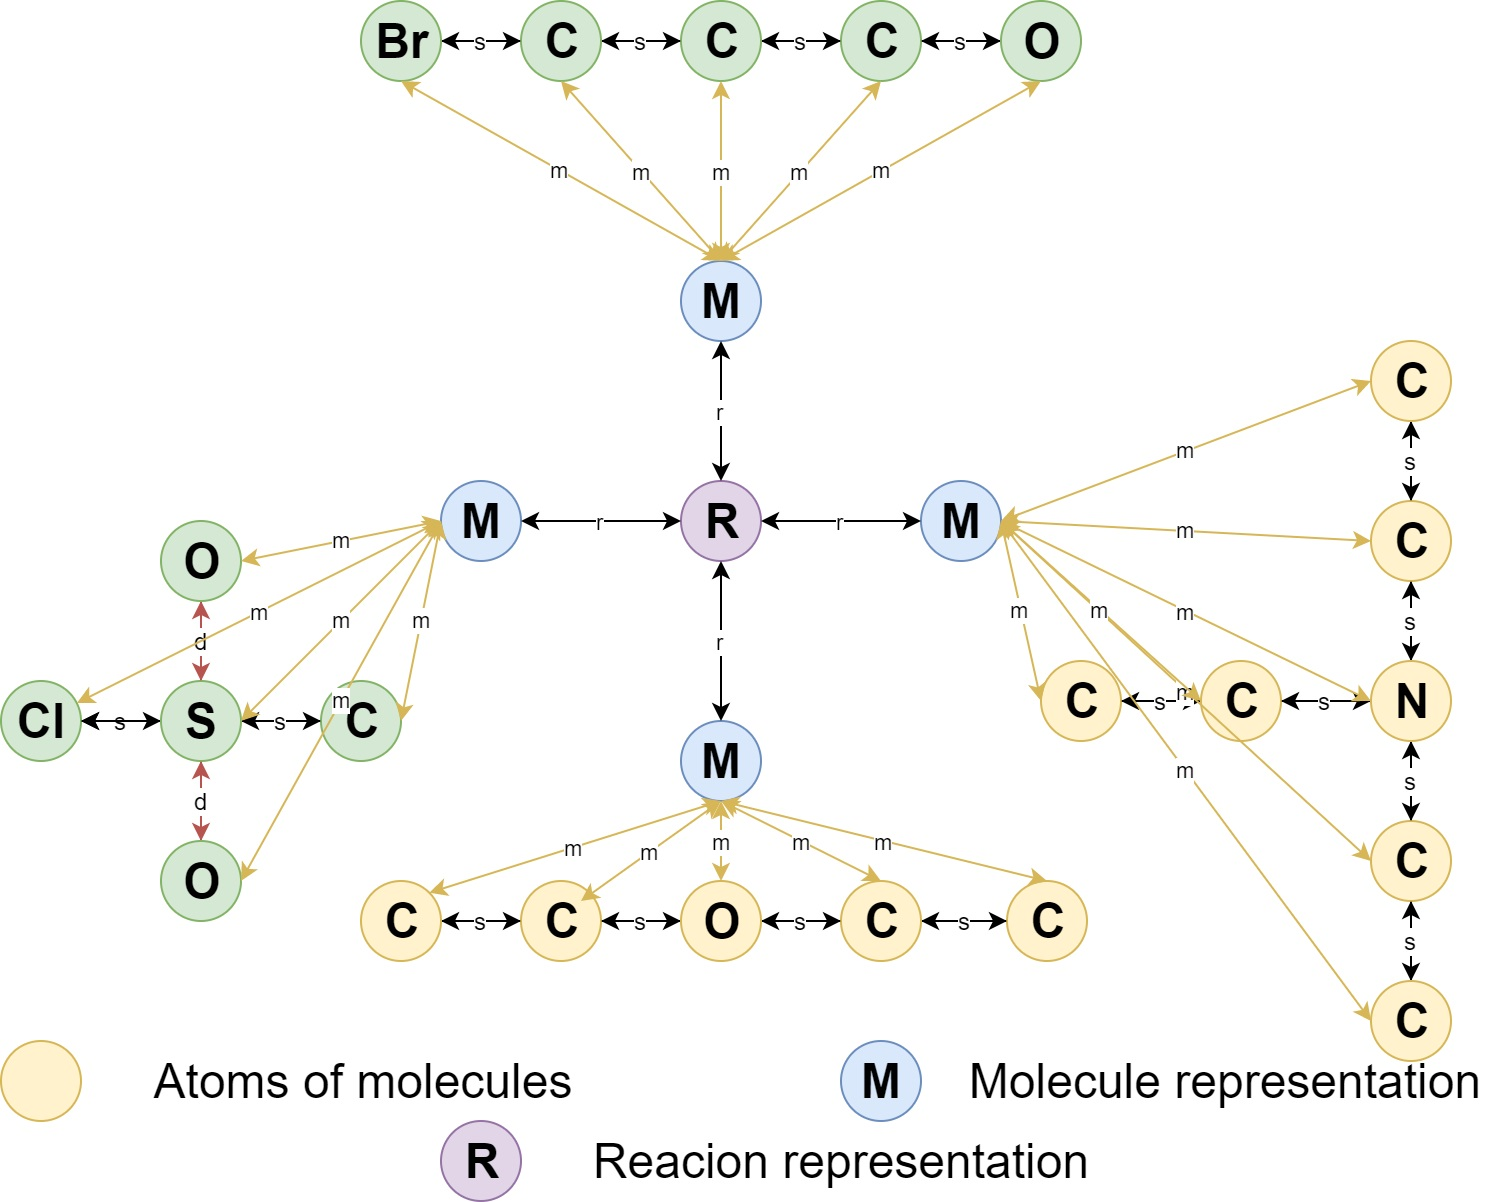
\includegraphics[width=0.8\textwidth]{images/supernode.jpg}
    \caption{Расширенный граф с введенными вершинами~--- представениями молекул и реакции}
    \label{fg:supernode_graph}
\end{figure}


\subsection{Агрегация графа.}

После прохождения RGCNN каждой реакции соответвует определенное число атомов, пусть $n$, тогда сделаем агрегацию графа.

\begin{equation}
    \mathbf{h}_g = \dfrac{1}{n}\sum_{i = 1}^{n}\mathbf{h}_i^{(m)},
\end{equation}

где $m$ -- количество слоев в RGCNN.

\subsection{Построение выхода сети}


Полученные векторные представления графов подаются на вход полносвязанной нейронной сети, решающей задачу регрессии~\eqref{eq:fcnn}
\begin{align}
    &\mathbf{h}_g^{(l+1)} = \text{ReLU}(\text{linear}(\mathbf{h}_g^{(l)}))\\
    &\hat{y} = \text{linear}({\mathbf{h}^{(t)}_g}),
    \label{eq:fcnn}
\end{align}

где $t$ -- количество слоев в полносвязанной нейронной сети.

\subsection{Функция ошибки}

В качестве функции ошибки была использована MSELoss, значение которой вычисляется следующим образом~\eqref{eq:loss}.

\begin{equation}
    \mathcal{L} = \dfrac{1}{n}\sum_{i = 1}^{n}\|y_i - \hat{y}_i\|_2^2
    \label{eq:loss}
\end{equation}

\section{Вычислительные эксперименты.}

Авторами редлагается несколько архитектур. Авторы приследуют две основные цели. Первая -- проверить, повышается ли качество модели при добавлении дополнительной информации о структуре графа. Вторая -- сравнить качество с с константной моделью.


Для начала проведения экспериментов необходимо найти в используемых выборках реакции, в которых известно поле \textbf{Mined Yield}. В результате этого каждая из выборок (train, test, valid) сокращается на $80\%$.
Поставленная задача является трудной. Во-первых, единственная доступная выборка содержит примеры всевозможных типов реакций. Во-вторых, после преобразований выборки становятся несбалансированными и неоднородными (см. Рис. \ref{fig:hist}). В-третьих, задача решается впервые,
поэтому для адекватной оценки модели в качестве простейшей выбрана константная \textbf{CONST} модель.
 

 \begin{figure}[h!]

\subfloat[Train]{
    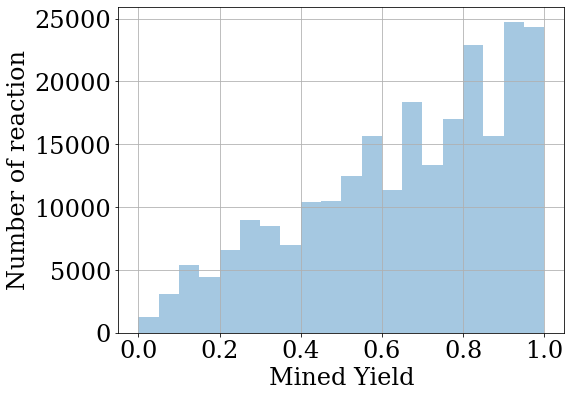
\includegraphics[width=0.35\textwidth]{images/train.jpg}}
\subfloat[Test]{
    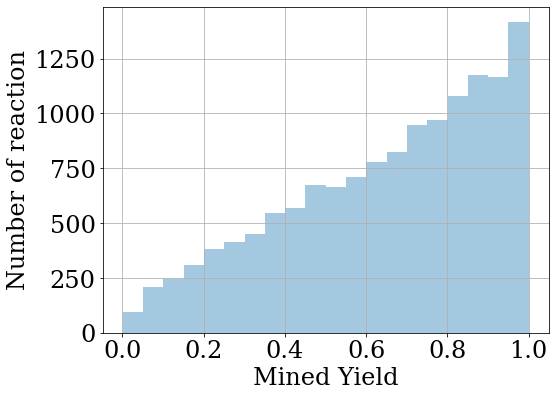
\includegraphics[width=0.35\textwidth]{images/test.jpg}}
\subfloat[Valid]{
    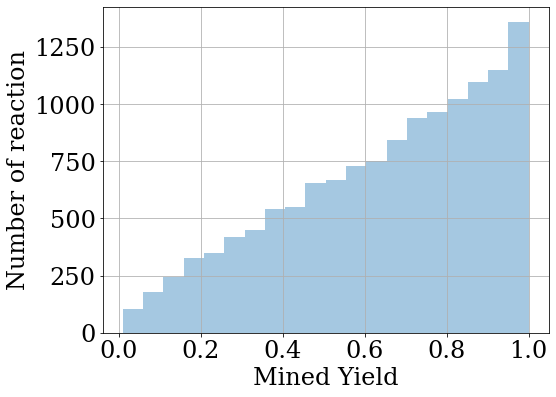
\includegraphics[width=0.35\textwidth]{images/valid.jpg}}
    
 \caption{\label{fig:hist} Распределение выходов реакций в каждой из выборок.}
\end{figure}


\subsection{Эксперименты}



\begin{table}[h!]
\caption{\label{tab:Models} Результаты экспериментов. $R^2$ -- коэффициент детерминации. $MAE$ -- среднее абсолютное отклонение между реальными выходами реакций и предсказанными на тестовой выборке. Коэффициент детерминации для константной модели не определен.}
\begin{center}
\begin{tabular}{|c|c|c|}
\hline
& \multicolumn{2}{c|}{\textbf{Mined Yield}} \\
\cline{2-3}
\raisebox{1.5ex}[0cm][0cm]{Модель}
& $R^2$ & $MAE$ \\
\hline
\textbf{CONST} & $0$ & $0.211 \pm 0.004$\\
\hline
\textbf{BASE} & $0.104 \pm 0.002$ & $0.198 \pm 0.003$ \\
\hline
\textbf{EG} & $0.125 \pm 0.003$ & $0.194 \pm 0.002$\\
\hline
\textbf{EGB} & $0.131 \pm 0.006$ & $0.186 \pm 0.002$\\
\hline
\textbf{EGBF} & $0.152 \pm 0.005$ & $0.174 \pm 0.003$\\
\hline
\end{tabular}
\end{center}

\end{table}


Базовая модель \textbf{BASE} состоит из двух частей: \textbf{RGCNN} и \textbf{FCNN} и принимает несвязанный граф исходных молекул. Предполагается, что известны только типы вершин. Данная модель не использует никакой специфичной информации (типы связей, свойства атомов) для конкретной задачи и не способна к передаче данных между компонентами(молекулами) в несвязанном графе. Модель демонстрирует самое низкое качество среди всех поставленных экспериментов(см. табл. \ref{tab:Models}), потому что конечное представление атома зависит только от представлений атомов в этой же молекуле. Однако основным механизмом химических реакций является именно межмолекулярное взаимодействие. 

 \begin{figure}[h!]
\subfloat[Loss]{
    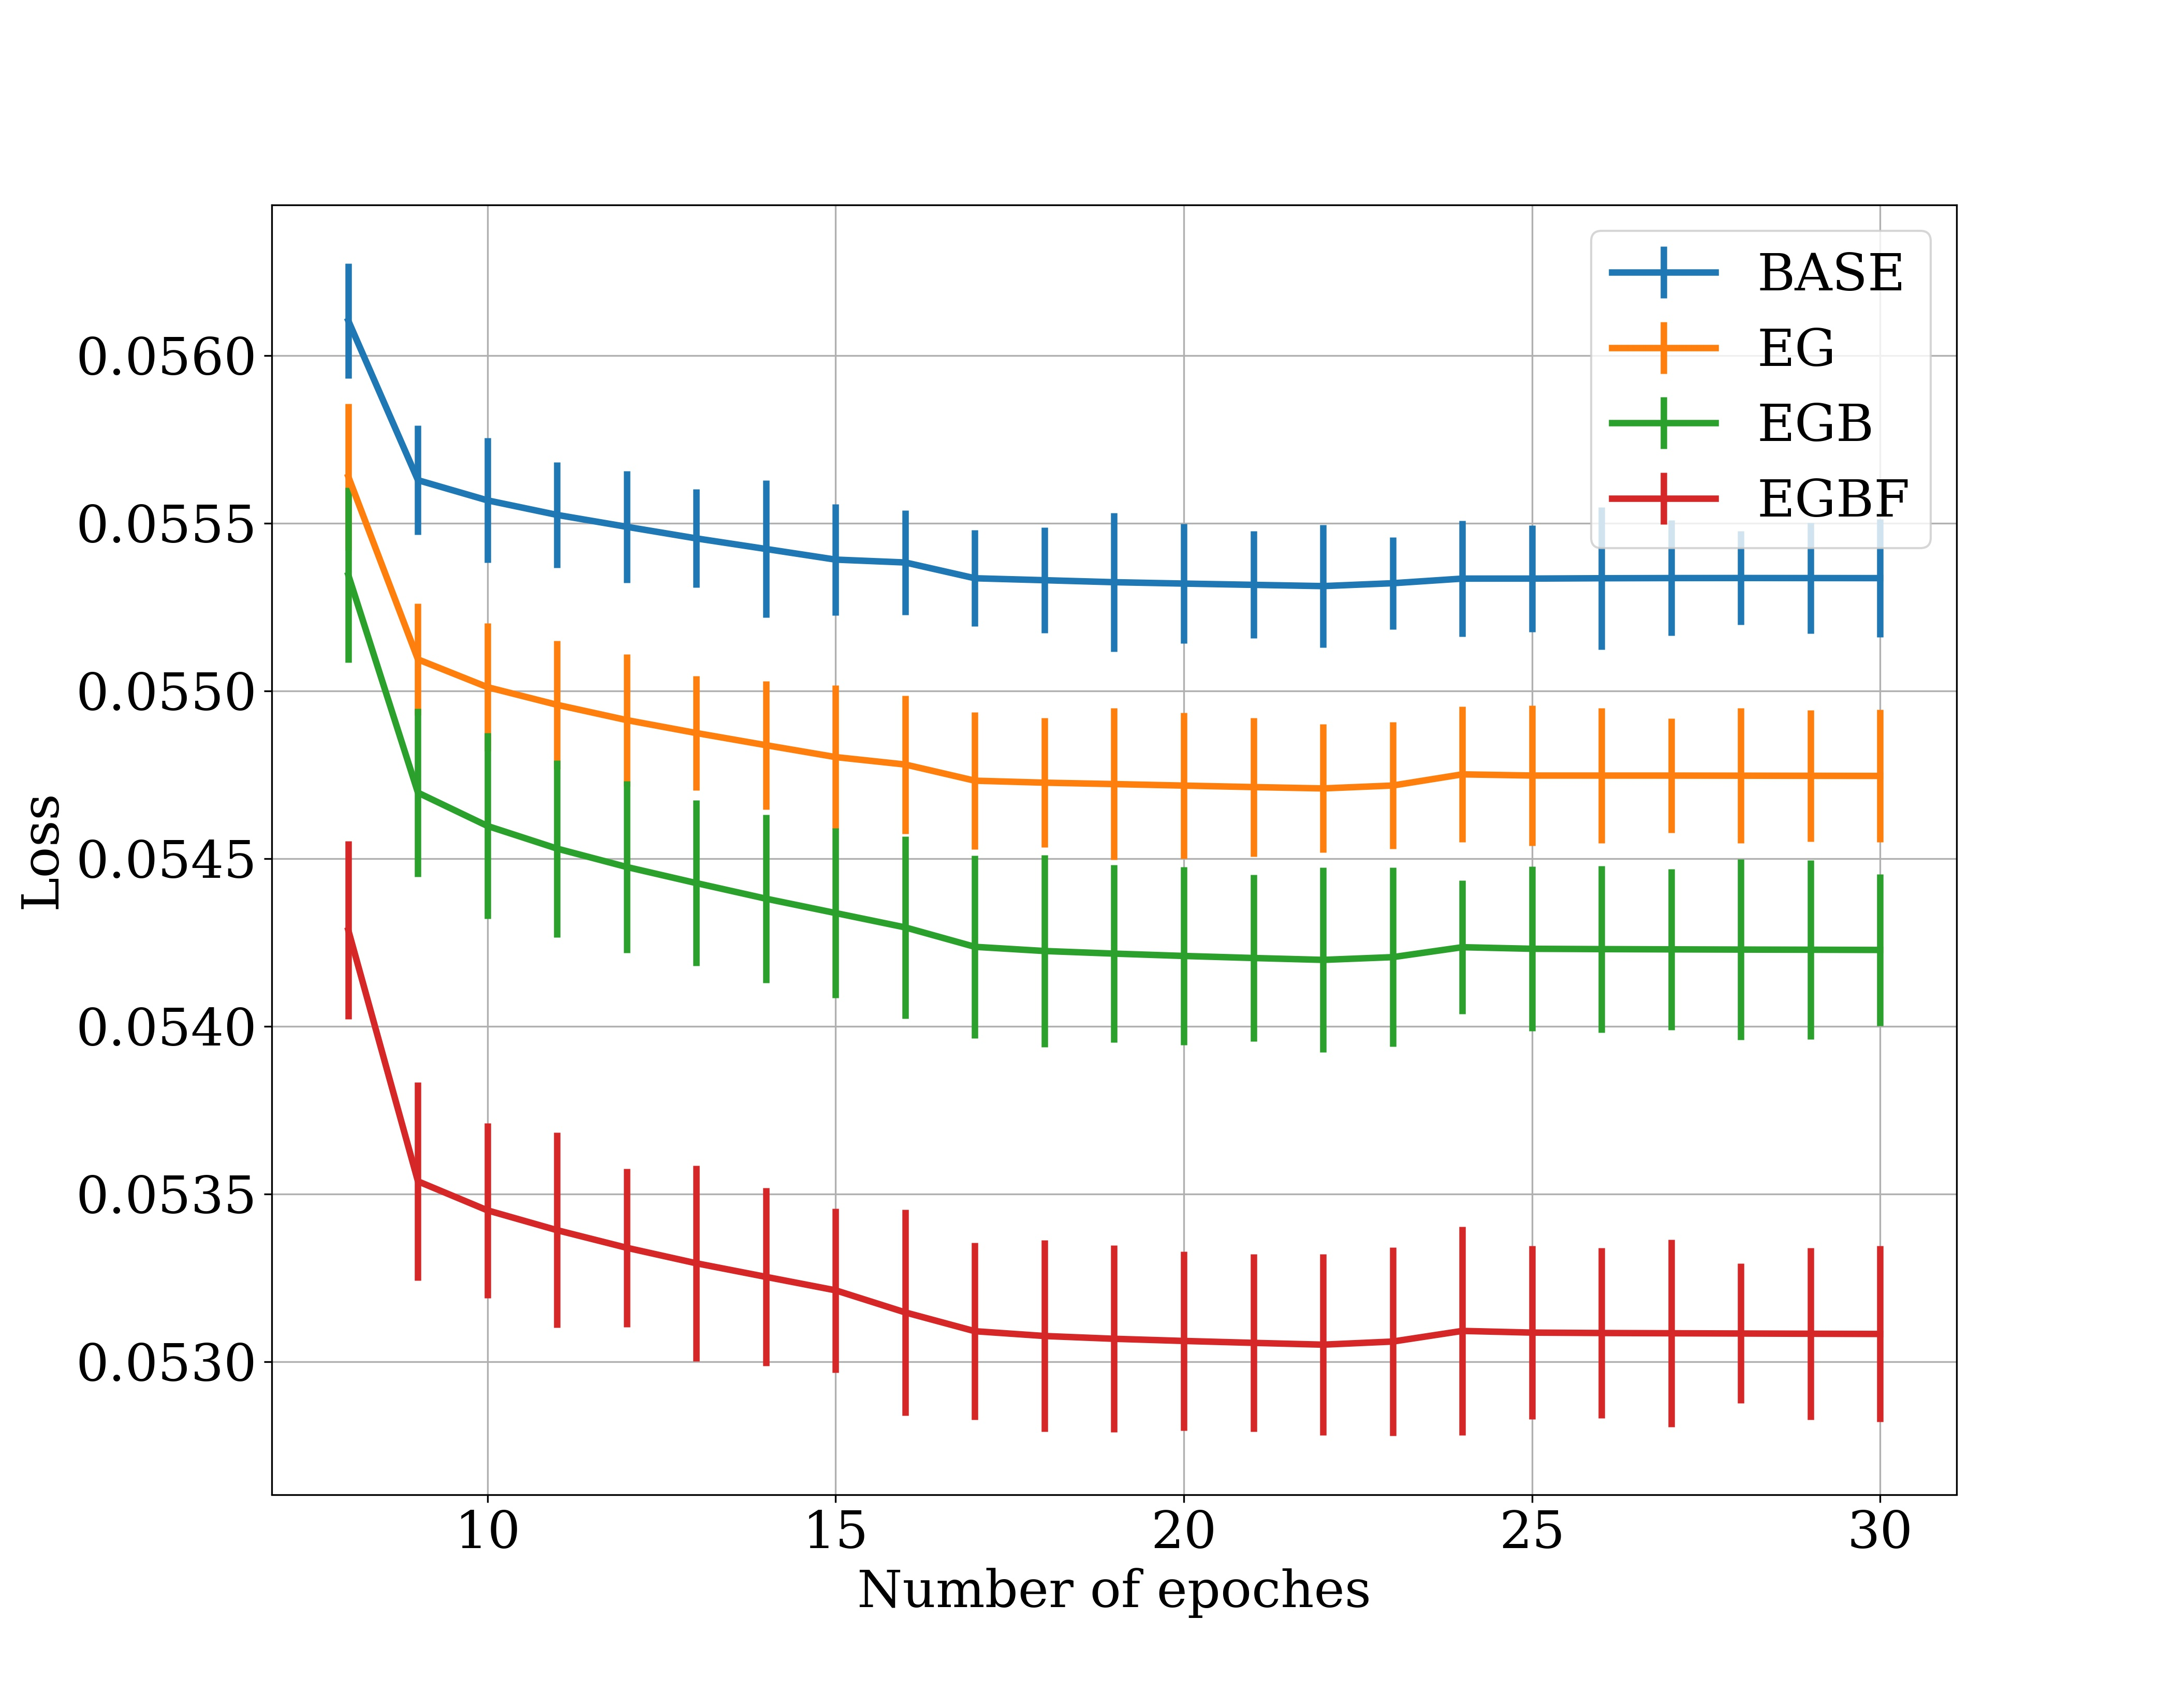
\includegraphics[width=0.52\textwidth]{images/com_graph(2).jpg}}
\subfloat[$R^2$]{
    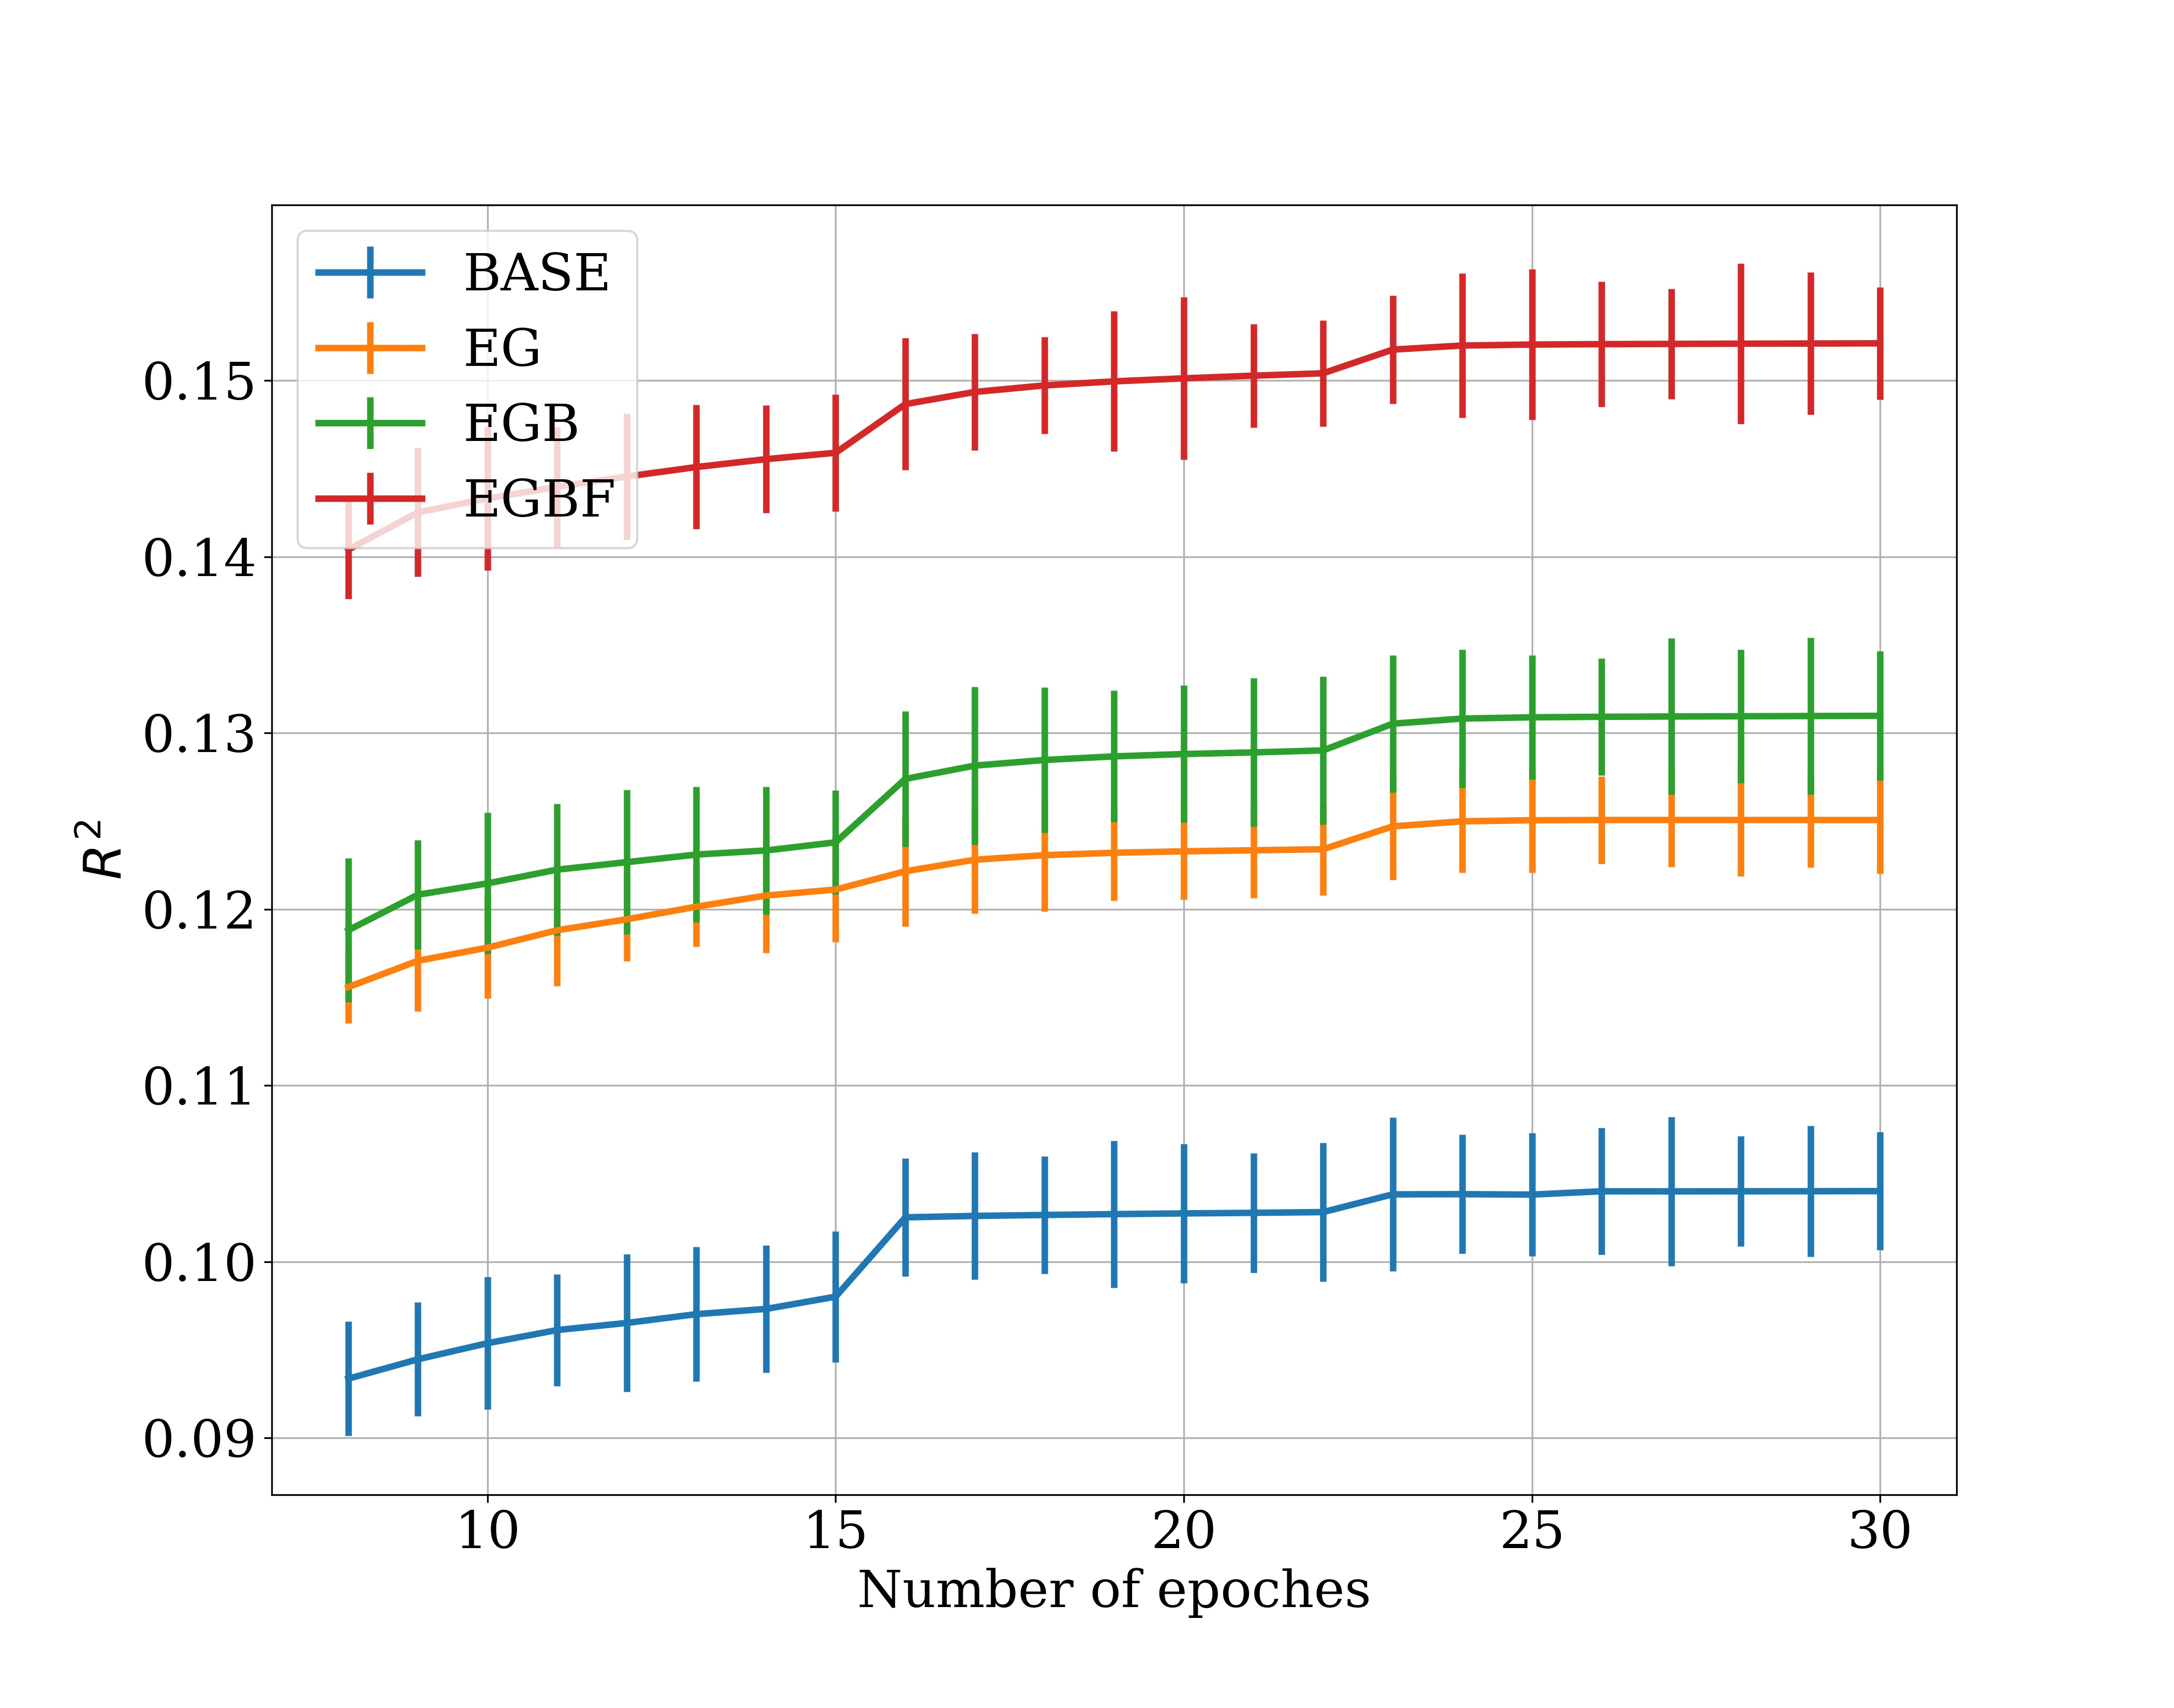
\includegraphics[width=0.52\textwidth]{images/com_graph_r2(2).jpg}}
    
 \caption{\label{fig:BASE} Результаты базового (\textbf{BASE}) эксперимента.Loss -- функция ошибки в процессе обучения, $R^2$ -- коэффициент детерминизации в процессе обучения между реальными значениями выхода тестовой выборки и предсказанными.}
\end{figure}




 Использование расширенного молекулярного графа \textbf{EG} в качестве входа \textbf{RGCNN} повышает качество модели. Повышение качества показывает, что дополнительное представление молекул и всей реакции моделирует межмолекулярное взаимодействие в химической реакции и обменивает информацию по исходным молекулярным графам. 
 
 Следующие модификации архитектуры заключаются в предоставлении дополнительной информации об атомах и связях. 
Эмбединги вершин содержат информацию о различных свойствах атома. Кроме того, реляционная структура сверточных слоев графа имитирует различные типы химических связей.
 
 Mодель \textbf{EGB} работает с различными типами химических связей: одинарными, двойными,тройными, ароматическими. Это приводит к повышению качества. 
 Наибольшее влияние на конечный результат оказывает использование различных расчетных свойств атомов при инициализации эмбедингов вершин в расширенном молекулярном графе. Свойства: степень, явная валентность, гибридизация, неявная валентность, ароматичность, неявность, число явных водородов, число неявных водородов, кольцо, число радикальных электронов, формальный заряд. Добавление этих  свойств в модель \textbf{EGBF} повышает качество модели. 
 
 
 Все эксперименты были проведены при помощи библиотек PyTorch~\cite{paszke2019pytorch} и DGL~\cite{wang2019deep}, запущены на Nvidia 1080 Ti. $30$ эпох обучения на лучшей архитектуре занимало примерно 6 часов.


\section{Выводы и планируемые исследования}

В данной работе построена регрессионная модель на множестве молекулярных графов. 
Проделанные эксперименты показали, что информация о структуре молекулярного графа повышает качество модели. Каждая из представленных архиктектур показала более высокое качество, чем константная модель. 
Дальнейшее улучшение модели возможно за счет обучения на выборке, в которой, во-первых, есть разделение на типы реакции, во-вторых, равномерное распределение выходов реакций. Также для увеличения качества регрессии предлагается классифицировать реакции по их типам.
.


\bibliography{literature}{}
\bibliographystyle{plain}

\end{document}
